%-----------------------------
% CSCI 315, Spring 2018
%
% <Gage Smith>
% Language: <Rust>
%-----------------------------


\documentclass{article}
%-----------------------------
% List of Packages
%-----------------------------
\usepackage{graphicx}   % Need for images
\usepackage{caption}     % Useful to suppress caption numbers with *
\usepackage{listings}      % Needed for code and syntax highlighting
\usepackage{minted}
\usepackage{multicol}     % Permits sections with multiple columns
\usepackage{enumitem}  % More options for itemize, enumerate, and description
\usepackage{hyperref}            % For nice urls
\usepackage{url}
\usepackage{tikz}            % For drawing cool things

%
%  You may add more packages as needed
%

%-----------------------------
% Set Settings and Macros
%-----------------------------

% define some custom colors
\definecolor{comment_green}{rgb}{0,0.6,0}
\definecolor{number_gray}{rgb}{0.5,0.5,0.5}
\definecolor{string_mauve}{rgb}{0.58,0,0.82}

% This is the default columnsep (from multicolums)
\setlength\columnsep{30pt}

%-----------------------------
\begin{document}
%-----------------------------
% Header
%-----------------------------
\title{Rust Fact Sheet \\ \large{\sc CSCI 315, Programming Languages}}
\author{Gage Smith}
\date{Spring 2019}
\maketitle


% Use tikz to add some images outside the normal printing area
\begin{tikzpicture}[remember picture,overlay]
  % This sets logo in upper right corner (optional)
  \node[anchor=north] at (current page.north)
              {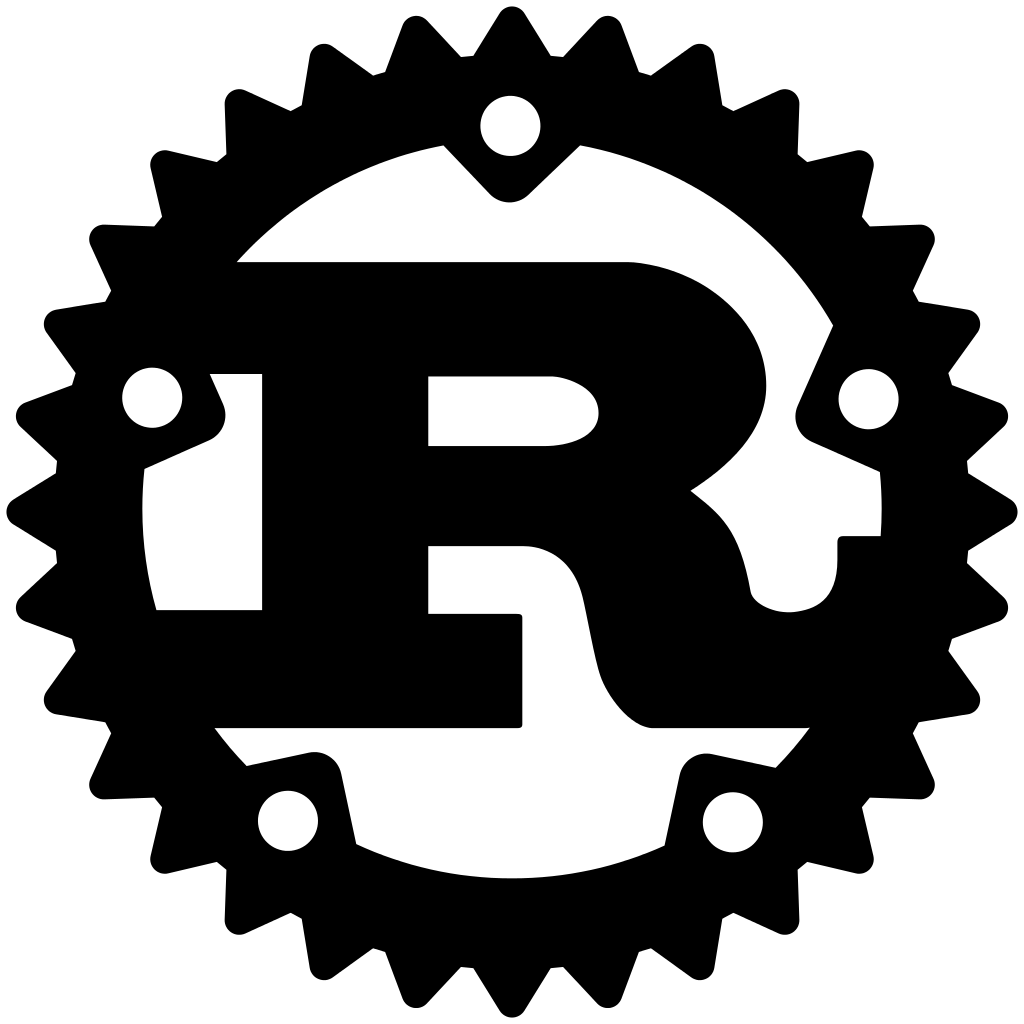
\includegraphics[scale=0.125]{img/rust_logo}};
\end{tikzpicture}


%-----------------------------
% Overview
%-----------------------------
\section*{Overview}
Rust is a programming language written by Graydon Hoare originally in 2006 while he was working for Mozilla Research. After its first stable release in 2015 it quickly became regarded as an open-source systems programming language. Rust focuses on speed, memory safety and parallelism. \cite{wiki:rust}

\noindent

%-----------------------------
% Version Information
%-----------------------------
\section*{Version History}
\textbf{Current Version:} 5.22.4, released July 15, 2017


% Tables show up where there is room. If having problems, look into the 'h' `t' or `p' designators
\begin{table}[b]
\label{revhistory}
\caption*{Rust: Major Revision History\cite{wiki:rust}}
\centering
\begin{tabular}{lll}
% \hline
\textbf{Year} & \textbf{Version} & \textbf{Note} \\
\hline
2006 & Pre-Release & Mozilla employee Graydon Hoare began Rust as a personal project. \\
2009-2010 & Pre-Release & Mozilla sponsored the project and announced it. \\
2011 & Pre-Release & First successful compilation with self-hosting compiler written in Rust. \\
2015 & 1.0 & First stable release of Rust v1.0. \\
2015 & 1.2 & Addition of classes. \\
2015 & 1.3 & Destructors and polymorphism through interfaces. \\
2015 & 1.4 & Traits added to have a means of inheritance. \\
2017 & 1.15 & Rust adopted the "open roadmap process". \\
2017 & 1.21 & Firefox Quantum begins utilizing a pure Rust CSS engine. \\
2017-2018 & 1.22-1.31.1 & Stack Overflow annual survey most loved programming language. \\
\end{tabular}
\end{table}



\newpage  % force a newpage, if desired
%--------------
%   Anatomy of a basic program
%--------------
\section*{Basics of Rust Programming\cite{code:rust}}
\subsubsection*{Declaring a Main()}
\begin{minted}{rust}
fn main()
{
    //Any amount of Rust code including other function declarations
}
\end{minted}

\subsubsection*{Intializing Variables}
\begin{minted}{rust}
    // Declare a variable binding
    let a_binding;

    {
        //Simple form
        let x = 2;

        // Initialize the binding
        a_binding = x * x;
    }
\end{minted}
\subsubsection*{Printing out Variables}
\begin{minted}{rust}
    // In general, the `{}` will be automatically replaced with any
    // arguments. These will be stringified.
    println!("{} days", 31);

    // Without a suffix, 31 becomes an i32. You can change what type 31 is,
    // with a suffix.

    // There are various optional patterns this works with. Positional
    // arguments can be used.
    println!("{0}, this is {1}. {1}, this is {0}", "Alice", "Bob");

    // As can named arguments.
    println!("{subject} {verb} {object}",
             object="the lazy dog",
             subject="the quick brown fox",
             verb="jumps over");

    // Special formatting can be specified after a `:`.
    println!("{} of {:b} people know binary, the other half doesn't", 1, 2);
\end{minted}

%-----------------------------
% Code Examples
%-----------------------------
\section*{Code Examples\cite{code:rust}}

\subsection*{Simple "Hello World"}
\begin{minted}{rust}
// This is the main function
fn main()
{
    // The statements here will be executed when the compiled binary is called

    // Print text to the console
    println!("Hello World!");
}

\end{minted}

\subsection*{Type Annotation and Primitives}
\begin{minted}{rust}
fn main()
{
    // Variables can be type annotated.
    let logical: bool = true;

    let a_float: f64 = 1.0;  // Regular annotation
    let an_integer   = 5i32; // Suffix annotation

    // Or a default will be used.
    let default_float   = 3.0; // `f64`
    let default_integer = 7;   // `i32`

    // A type can also be inferred from context
    let mut inferred_type = 12; // Type i64 is inferred from another line
    inferred_type = 4294967296i64;

    // A mutable variable's value can be changed.
    let mut mutable = 12; // Mutable `i32`
    mutable = 21;

    // Error! The type of a variable can't be changed.
    mutable = true;

    // Variables can be overwritten with shadowing.
    let mutable = true;
}

\end{minted}

\newpage
\subsection*{Working With Block Expressions}
\begin{minted}{rust}
fn main() {
    let x = 5u32;

    let y = {
        let x_squared = x * x;
        let x_cube = x_squared * x;

        // This expression will be assigned to `y`
        x_cube + x_squared + x
    };

    let z = {
        // The semicolon suppresses this expression and `()` is assigned to `z`
        2 * x;
    };

    println!("x is {:?}", x);
    println!("y is {:?}", y);
    println!("z is {:?}", z);
}
\end{minted}

\subsection*{General If-Else Structure}
\begin{minted}{rust}
fn main() {
    let n = 5;

    if n < 0 {
        print!("{} is negative", n);
    } else if n > 0 {
        print!("{} is positive", n);
    } else {
        print!("{} is zero", n);
    }
}

\end{minted}


%-----------------------------
% Applications
%-----------------------------
\section*{Useful Applications\cite{info:rust}}

\begin{itemize}[noitemsep]
\item Systems programming
\item Command Line Interfaces (CLI)
\item Web Assembly
\item Utilizing type system for Networking interfaces
\item Game Emulation/Game Development
\item Package Management Software
\end{itemize}
\bigskip     % add some space, but more than \smallskip or \medskip






\bigskip     % add some space, but more than \smallskip or \medskip
\bigskip     % add some space, but more than \smallskip or \medskip

\section*{Cargo Build System Tutorial/Overview\cite{code:rust}}
Rust has a build system and package manager called ''Cargo''. Cargo allows for simple and easy downloading/building libraries for your Rust code to run upon.
\begin{minted}{bash}
#Check your version number
$ cargo --version

#Move your source files in to a "src" directory
$ mkdir src
$ mv main.rs src/main.rs
$ rm main

#Make a Cargo configuration file .toml
#Place this file in your project directory that contains the "src" directory
#Must have a capitalized 'C'

$touch Cargo.toml
\end{minted}

\begin{minted}{yaml}
#Add to Cargo.toml
[package]

name = "hello_world"
version = "0.0.1"
authors = [ "Your name <you@example.com>" ]

\end{minted}

\begin{minted}{bash}
#Simple build and run commands with Cargo
$ cargo build
$ cargo run
\end{minted}
%-----------------------------
% Fun Facts
%-----------------------------
\section*{Interesting Factoids\cite{wiki:rust}}

\begin{enumerate}
\item Rust was originally named after a fungus called rust.

\item Rust was nominated ''most loved programming language'' in Stack Overflow Developer Survey three years straight from 2016 to 2018.

\item There is a list of \href{https://github.com/rust-unofficial/awesome-rust#games}{games*} completely composed of Rust.
\end{enumerate}



%-----------------------------
% Quick Facts
%-----------------------------
\section*{Quick Reference\cite{wiki:rust}}

% minipage can be used to space out smaller sections (often side by side in 2 columns)
% here we make a 3/4 page and center it
\begin{center}
\begin{minipage}[c]{0.75\linewidth}
\begin{description}[noitemsep]
\item [URL:] \url{www.rust-lang.org}
\item [Extension:] \texttt{.rs .rlib}
\item [Operating System:] cross-platform
\item [Written in:] Rust/OCaml
\item [Paradigm:] multi-paradigm \\(imperative, functional, concurrent)
\item [Typing:] Static, Strong, Linear
\item [Appeared:] 2010
\item [Age in 2018:] 8
\item [Created by:] Graydon Hoare
%\item [Corporate Support:]  if any
\item [Influenced by:] C\#, C++, Haskell, OCaml, Scheme, Swift
\item [Canonical Text]: \textsl{Programming Rust: Fast, Safe Systems Development} (2017)
\end{description}
\end{minipage}
\end{center}
\bigskip     % add some space, but more than \smallskip or \medskip


%-----------------------------
% Relevant XKCD or other comic (optional)
%-----------------------------
\section*{}
\medskip
\begin{center}
    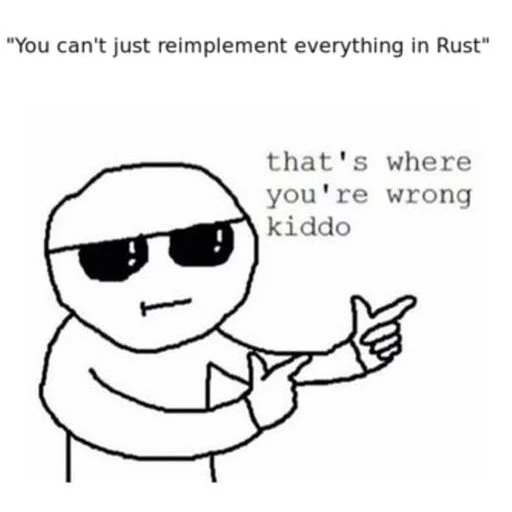
\includegraphics[width=0.8\textwidth]{img/rust_comic}
\end{center}
\bigskip     % add some space, but more than \smallskip or \medskip
\bigskip     % add some space, but more than \smallskip or \medskip
\newpage
%-----------------------------
% References (Required)
%-----------------------------
\bibliographystyle{plain}
\bibliography{Rust}      % matches rust.bibs


%-----------------------------
\end{document}
%-----------------------------;
